\documentclass{beamer} %

%%%BASICS
\usepackage[utf8]{inputenc}
\usepackage{csquotes}

%%%START THEME SETTINGS
\usetheme{Madrid}
\usefonttheme{professionalfonts}

%%%END THEME SETTINGS

%%%START APA
\usepackage[british]{babel}

% ____ Bibliography ____
\usepackage{natbib} %Bibliography.
% \setcitestyle{numbers} %Cite as numbers or author-year.
\bibliographystyle{plain} %Reference style.
% ______________________

% Confusion Matrix
\usepackage{array}
\usepackage{multirow}
\newcommand\MyBox[2]{
  \fbox{\lower0.75cm
    \vbox to 1.7cm{\vfil
      \hbox to 1.7cm{\centering \hfil\parbox{0.5cm}{#1\\#2}\hfil}
      \vfil}%
  }%
}

% Tables
\usepackage{array}
\newcolumntype{C}[1]{>{\centering\arraybackslash}m{#1}}

%% APA citing
%% \cite{t} - Uthor und Richter, 2010
%% \textcite{t} - Uthor und Riter (2010)
%% \parencite{t} - (Uthor & Riter, 2010)
%% \parencite[Chapt.~4]{t} - (Uthor & Riter, 2010, S. 15)
%%%END APA


\title[Meta-labeling]{Chapter 1: Meta-labeling}
\institute[HKUST - UPC]{HKUST - UPC}
\author{Guillermo Creus}

\date{\today}

\begin{document}

\begin{frame}
	\titlepage
\end{frame}

%------------------------------------------------------


\begin{frame}{Idea}
Imagine you were dealing with a financial time series 
and you wanted to predict the \textbf{side} (long/short or 
pass) and \textbf{size} of your investment. If the explanatory variables of \textbf{side} are different, then meta-labeling is useful:
	
	\begin{block}{\centering Primary Model (M1)}
	\begin{itemize}
		\item Labels: $y_{\text{M1}} \in \{-1, 1\}$. A positive is 
		understood as the model telling you to open a position.
	\end{itemize}
	\end{block}
	
	\begin{block}{\centering Secondary Model (M2)}
	Its main function is to decide if a positive from the primary 
	model is a true positive (i.e. whether to trade with the side 
	of M1)
	\begin{itemize}
		\item Features: $\hat{y}_{\text{M1}}$ and same or different 
		set of features than model 1.
		\item Labels: $y_{\text{M2}} = 1 \ \text{if} \ 
		\hat{y}_{\text{M1}} = y_{\text{M1}},\ 0 \ 
		\text{otherwise}$.
		\item \textbf{TP:} profitable investment, \textbf{FP:} losing 
		investment, 	\textbf{TN:} M2 predicts correctly that M1 was 
		wrong, \textbf{FN:} M2 predicts M1 was wrong when the latter 
		was right.
	\end{itemize}
	\end{block}
\end{frame}

\begin{frame}{Toy Project}
	The main idea of this project was to determine how meta-labeling 
	works with synthetic data. In this case, 5 features have been 
	used: $\textbf{X}_{\cdot, 1}, \ 
	\textbf{X}_{\cdot, 2}$ (M1) and 
	$\textbf{X}_{\cdot, 3},\ 
	\textbf{X}_{\cdot, 4},\ 
	\textbf{X}_{\cdot, 5}$ (M2).\\
	
	\begin{itemize}
		\item $\textbf{X}_{k, i} \sim N(\mu_i,\ \sigma^2)$
		\item $\omega_k = \textbf{sigmoid} \left( \alpha + 
		\sum_{i = 1}^{5} \textbf{X}_{k,i} \cdot \beta_i + \epsilon_k 
		\right)$ where $\epsilon_k \sim N(0,\ \sigma_{\epsilon}^2)$ 
		and $\textbf{sigmoid}(z) = \frac{1}{1 + e^{-z}}$
	\end{itemize}
	
	\vspace{.2cm}
	
	The labels are defined as:

	\begin{equation*}
		y_k^{\text{M1}} =
	    \begin{cases}
	      -1 & \text{if}\ \omega_k < 0.5 \\
	      \hfill 1 & \text{otherwise} 
	    \end{cases}
	\end{equation*}
\end{frame}

\begin{frame}{Toy Project}
  \framesubtitle{Definition of Models}
  
  \begin{columns}
    \begin{column}{.45\textwidth}
        \begin{block}{Primary Model}
        		\begin{itemize}
        			\item \textbf{Features:} $\textbf{X}_1,\ \textbf{X}_2$
        			\item \textbf{Labels:} $y^{\text{M1}}$
        			\item \textbf{Model:} Neural Network (1 layer) for 
        			Binary Classification
        		\end{itemize}
        \end{block}
    \end{column}

    \begin{column}{.45\textwidth}
        \begin{block}{Secondary Model}
			\begin{itemize}
        			\item \textbf{Features:} $\textbf{X}_3,\ \textbf{X}_4,
        			\ \textbf{X}_5,\ \hat{y}^{\text{M1}}$
        			
        			\item \textbf{Labels:} $y^{\text{M2}}$
        			
					\vspace{.1cm}        			
        				\scalebox{0.5}{
					$
						y_k^{\text{M2}} =
					    \begin{cases}
					      1 & \text{if}\ \hat{y}^{\text{M1}}_k = 
					      y^{\text{M1}}= -1\ \text{or}\ 
					      \hat{y}^{\text{M1}}_k = 
					      y^{\text{M1}}= 1\\
					      \hfill 0 & \text{otherwise} 
					    \end{cases}
					$ 
					} 
					
        			\item \textbf{Model:} Neural Network (1 hidden layer - 
        			Leaky ReLU) for Binary Classification
        			
        		\end{itemize}
        \end{block}
    \end{column}
    
  \end{columns}
	
\end{frame}

\begin{frame}{Toy Project}
\framesubtitle{Results}

  \begin{columns}
    \begin{column}{.45\textwidth}
        \begin{block}{Primary Model}
        		\centering
        		\scalebox{0.65}{
			\renewcommand\arraystretch{1.5}
			\setlength\tabcolsep{0pt}
			\begin{tabular}{c >{\bfseries}r @{\hspace{0.7em}}c @{\hspace{0.4em}}c @{\hspace{0.7em}}l}
			  \multirow{10}{*}{\parbox{1.1cm}{\bfseries\raggedleft Actual\\ value}} & 
			    & \multicolumn{2}{c}{\bfseries Prediction outcome} & \\
			  & & \bfseries 1 & \bfseries 0 & \bfseries Total \\
			  & 1 & \MyBox{TP}{115} & \MyBox{FN}{0} & 115 \\[2.4em]
			  & 0 & \MyBox{FP}{85} & \MyBox{TN}{0} & 85 \\
			  & Total & 200 & 0 &
			\end{tabular}}
        \end{block}
    \end{column}
    
    \begin{column}{.45\textwidth}
        \begin{block}{Secondary Model}
        		\centering
        		\scalebox{0.65}{
			\renewcommand\arraystretch{1.5}
			\setlength\tabcolsep{0pt}
			\begin{tabular}{c >{\bfseries}r @{\hspace{0.7em}}c @{\hspace{0.4em}}c @{\hspace{0.7em}}l}
			  \multirow{10}{*}{\parbox{1.1cm}{\bfseries\raggedleft Actual\\ value}} & 
			    & \multicolumn{2}{c}{\bfseries Prediction outcome} & \\
			  & & \bfseries 1 & \bfseries 0 & \bfseries Total \\
			  & 1 & \MyBox{TP}{105} & \MyBox{FN}{10} & 115 \\[2.4em]
			  & 0 & \MyBox{FP}{49} & \MyBox{TN}{36} & 85 \\
			  & Total & 154 & 46 &
			\end{tabular}}
        \end{block}
    \end{column}

  \end{columns}

	\vspace{.3cm}
	Remember that Actual Value $= 1 \Rightarrow$ Trade and Actual 
	Value $= 0 \Rightarrow$ Don't trade 	
	
\end{frame}

\begin{frame}{Toy Project}
\framesubtitle{Metrics}

	\begin{figure}
	\centering
		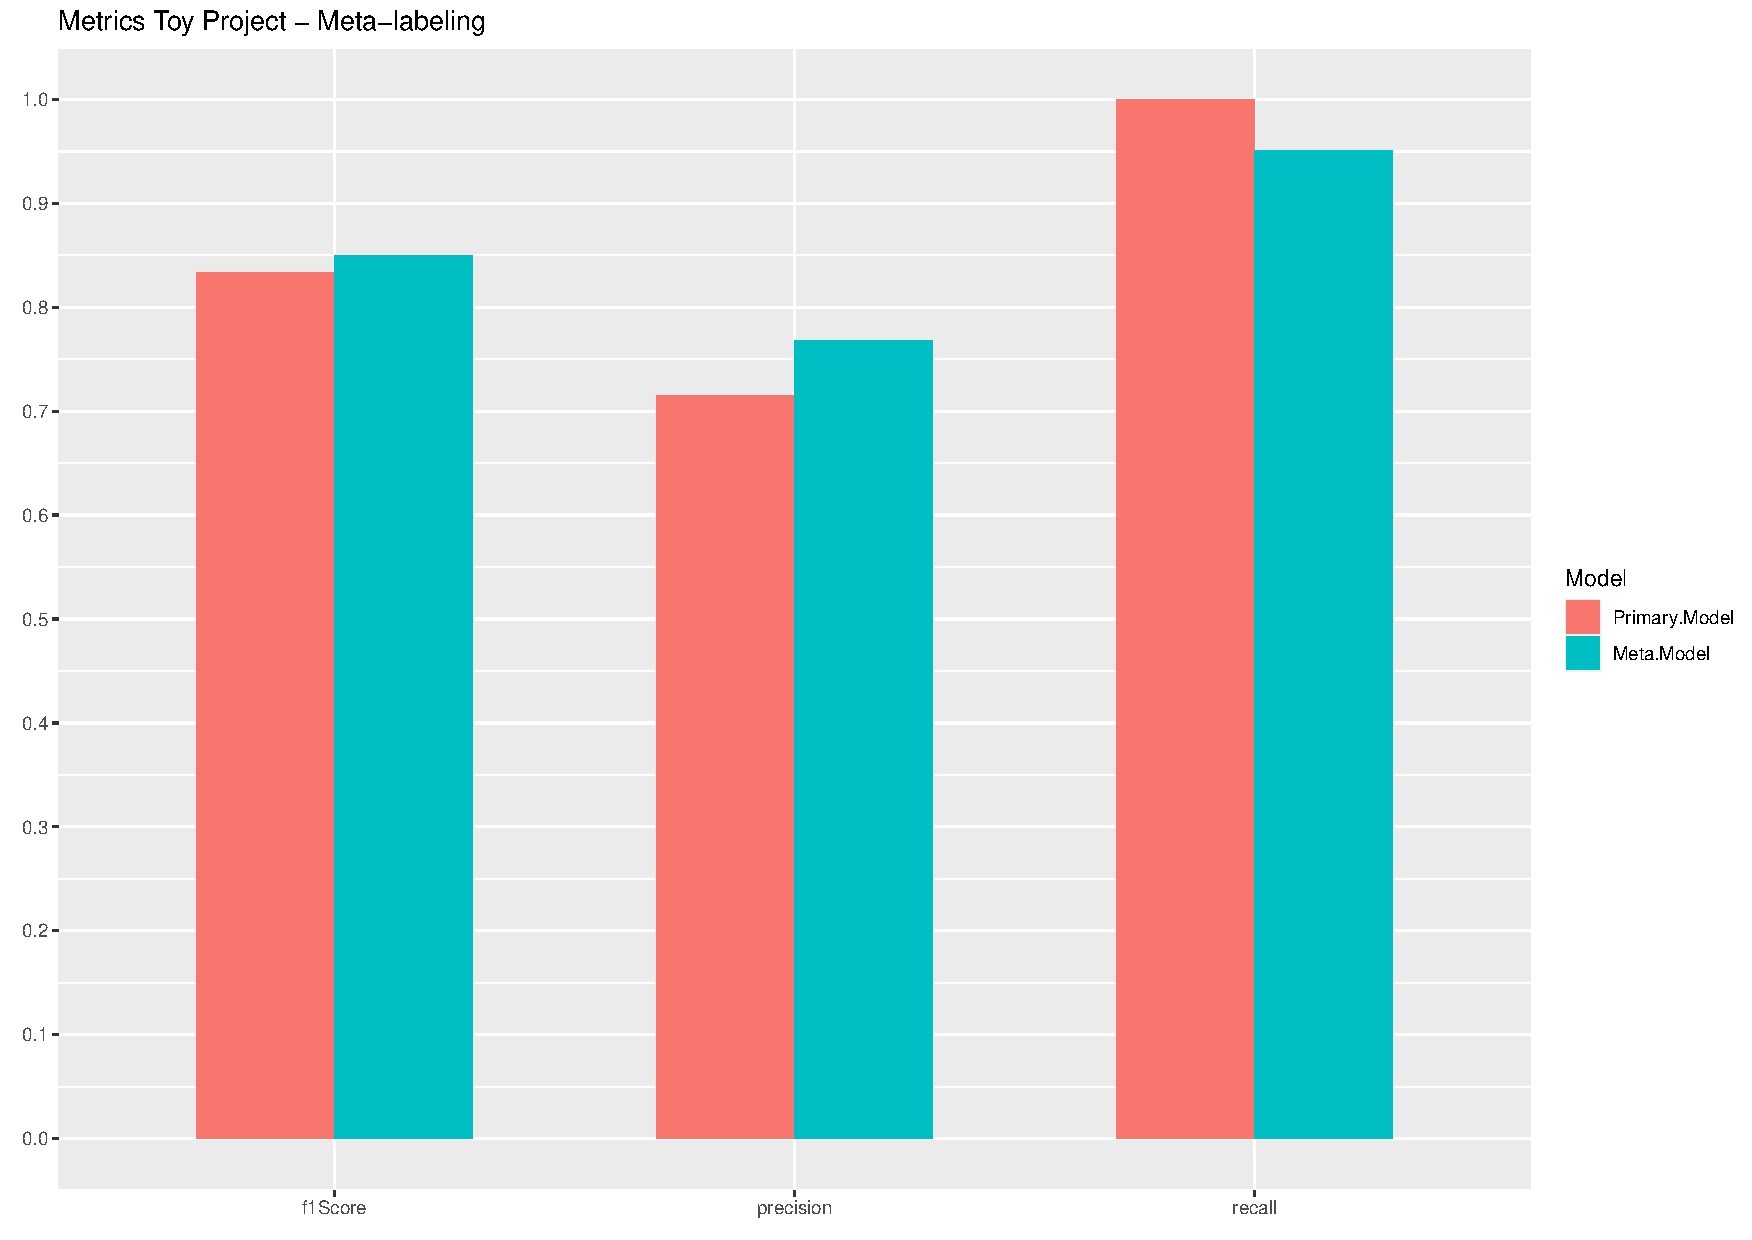
\includegraphics[scale=.275]{../img/toyProjectMetrics}
	\end{figure}
	
	The high recall of the Primary Model brought many False Positives 
	which have been corrected in the Meta Model (Primary + Secondary 
	Model). That is why the F1-Score of the Meta Model is higher.
\end{frame}

\begin{frame}{Labeling in financial time series}
\framesubtitle{Triple Barrier Method}

	\begin{itemize}
		\item \textbf{Horizontal barriers:} Dynamic levels that depend 
		on the 10 day rolling volatility and the price at the first 
		day considered. They can be symmetric or not.
		\item \textbf{Vertical barrier:} Set as a fixed time horizon. 
		In this case, 10 days.
	\end{itemize}
	
	\begin{columns}
	\begin{column}{.45\textwidth}
		\begin{figure}[htbp]
			\centering
			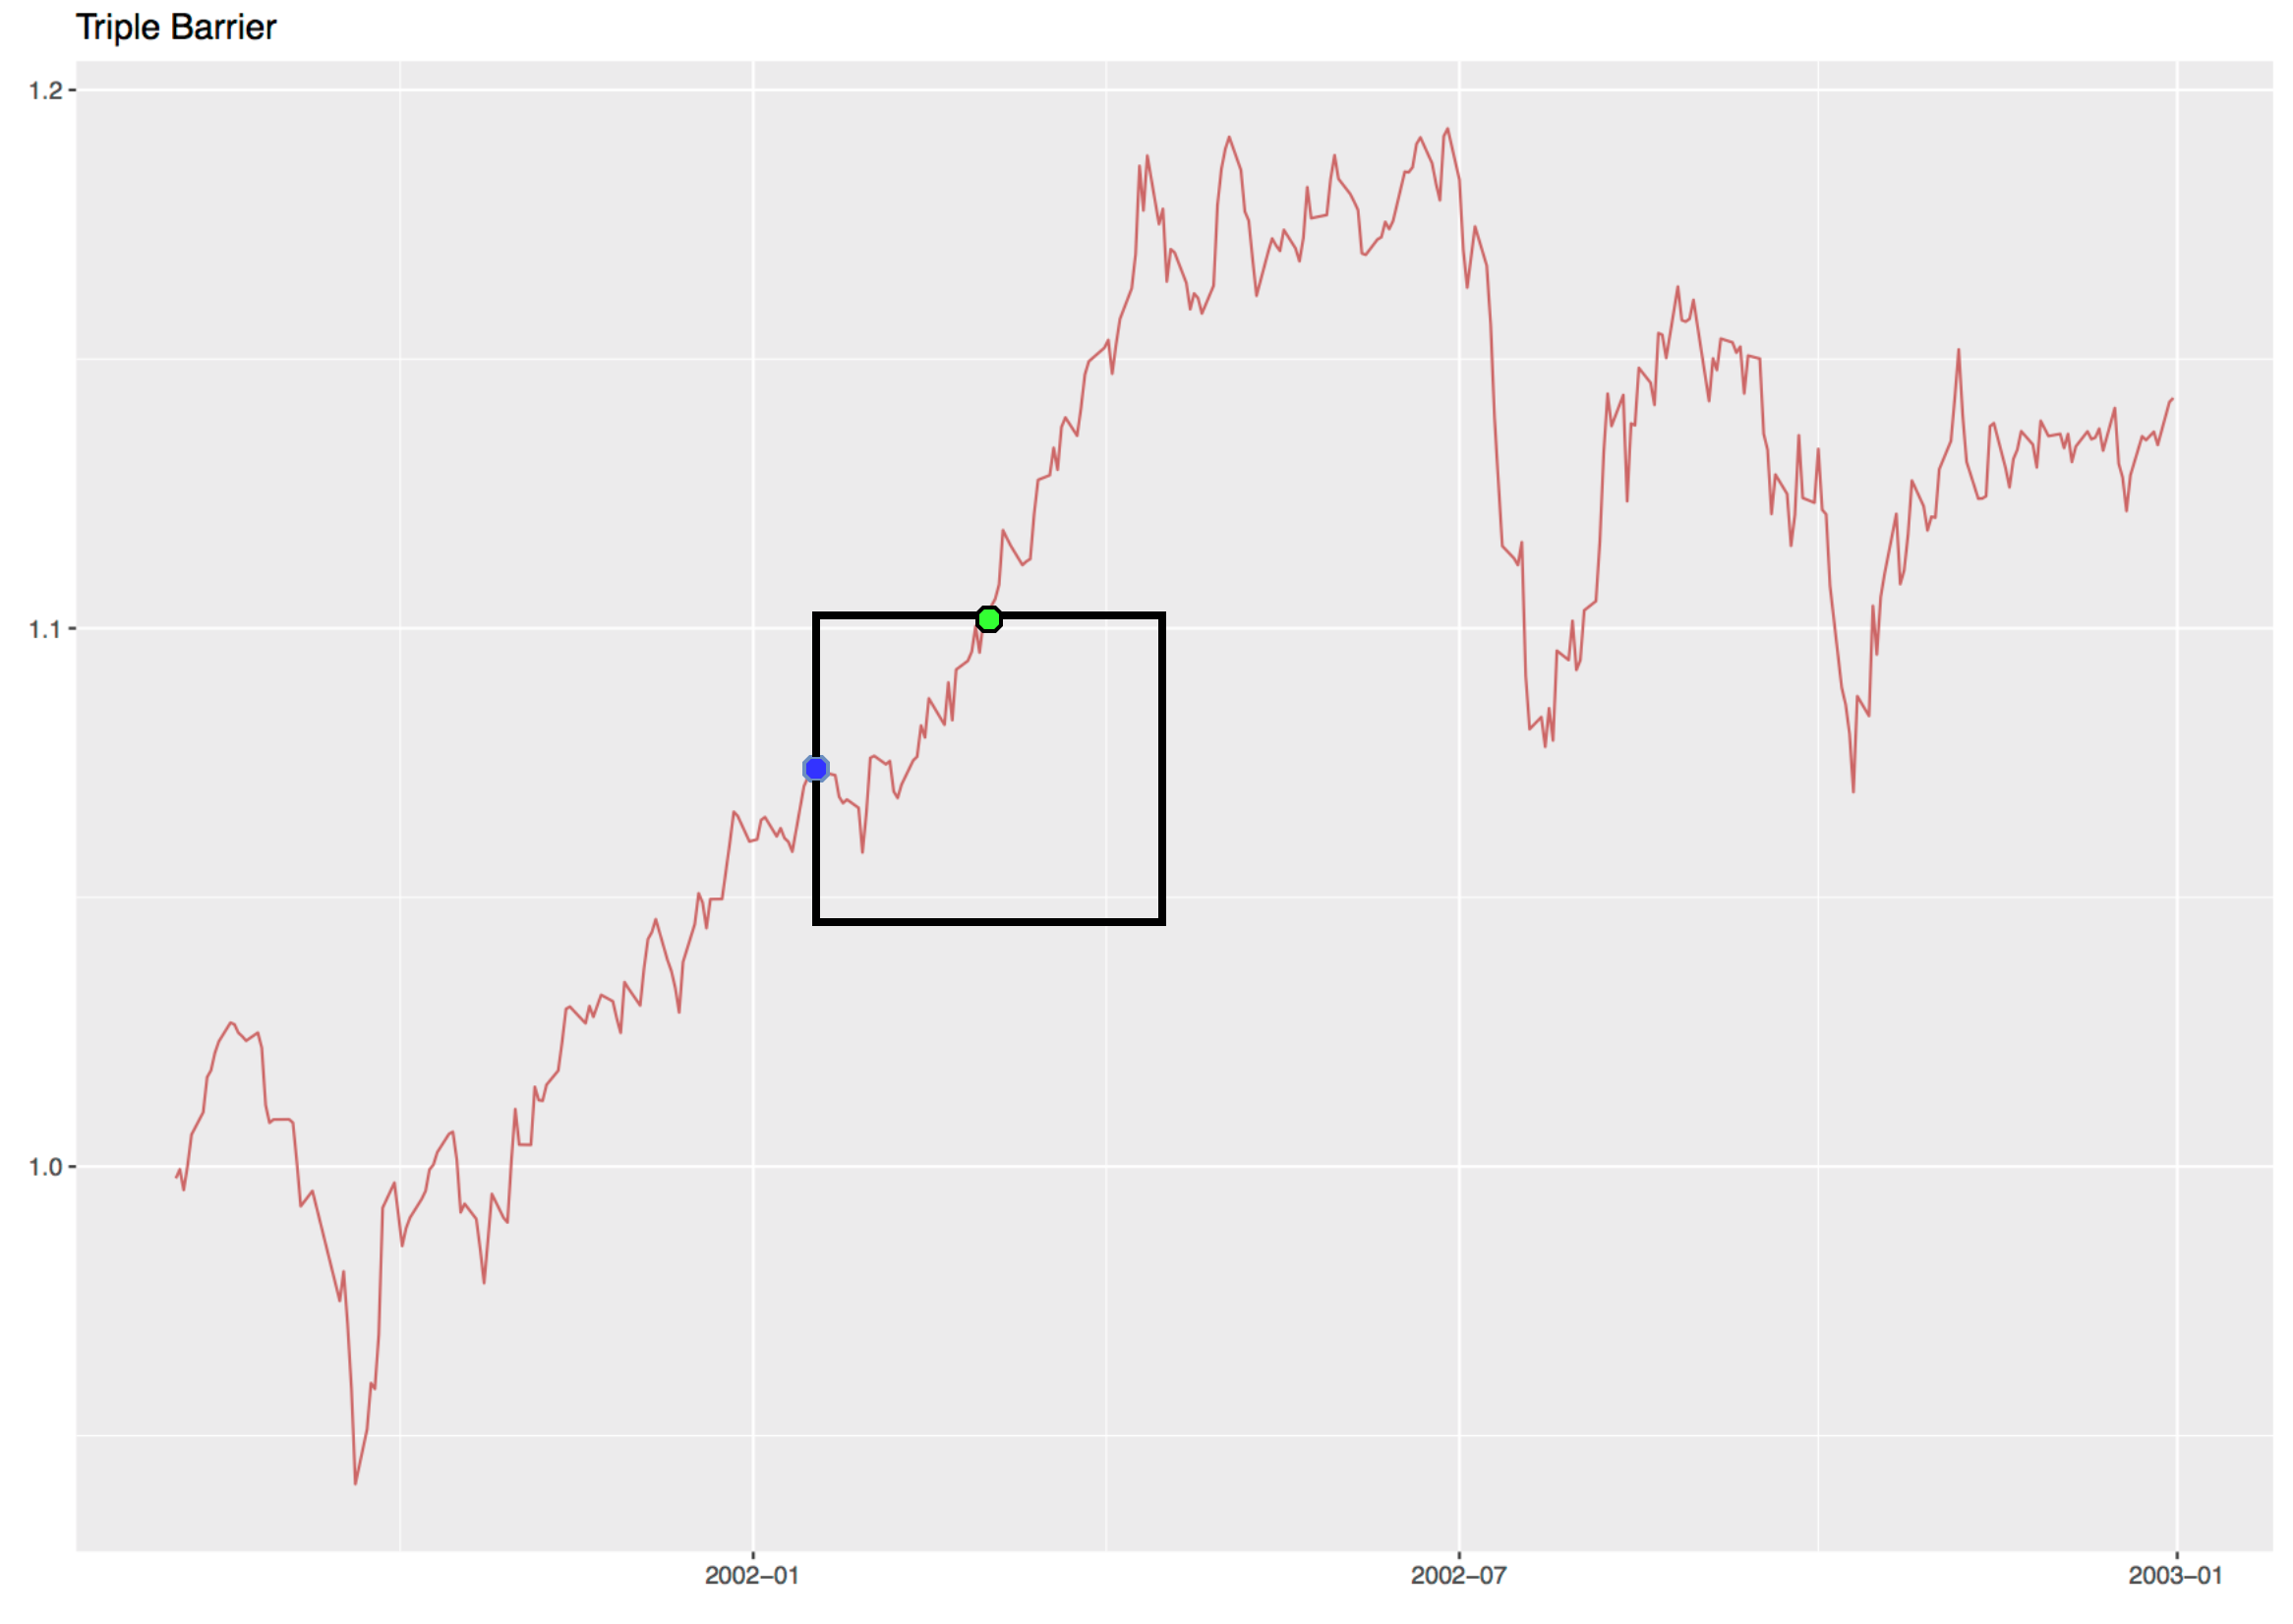
\includegraphics[width=.9\textwidth]
			{../img/tripleBarrierSymmetric.png}
			\caption{Symmetrical horizontal barriers}
			\label{fig:tripleBarrierSide}
		\end{figure}
	\end{column}
	
	\begin{column}{.45\textwidth}
		\begin{figure}[htbp]
			\centering
			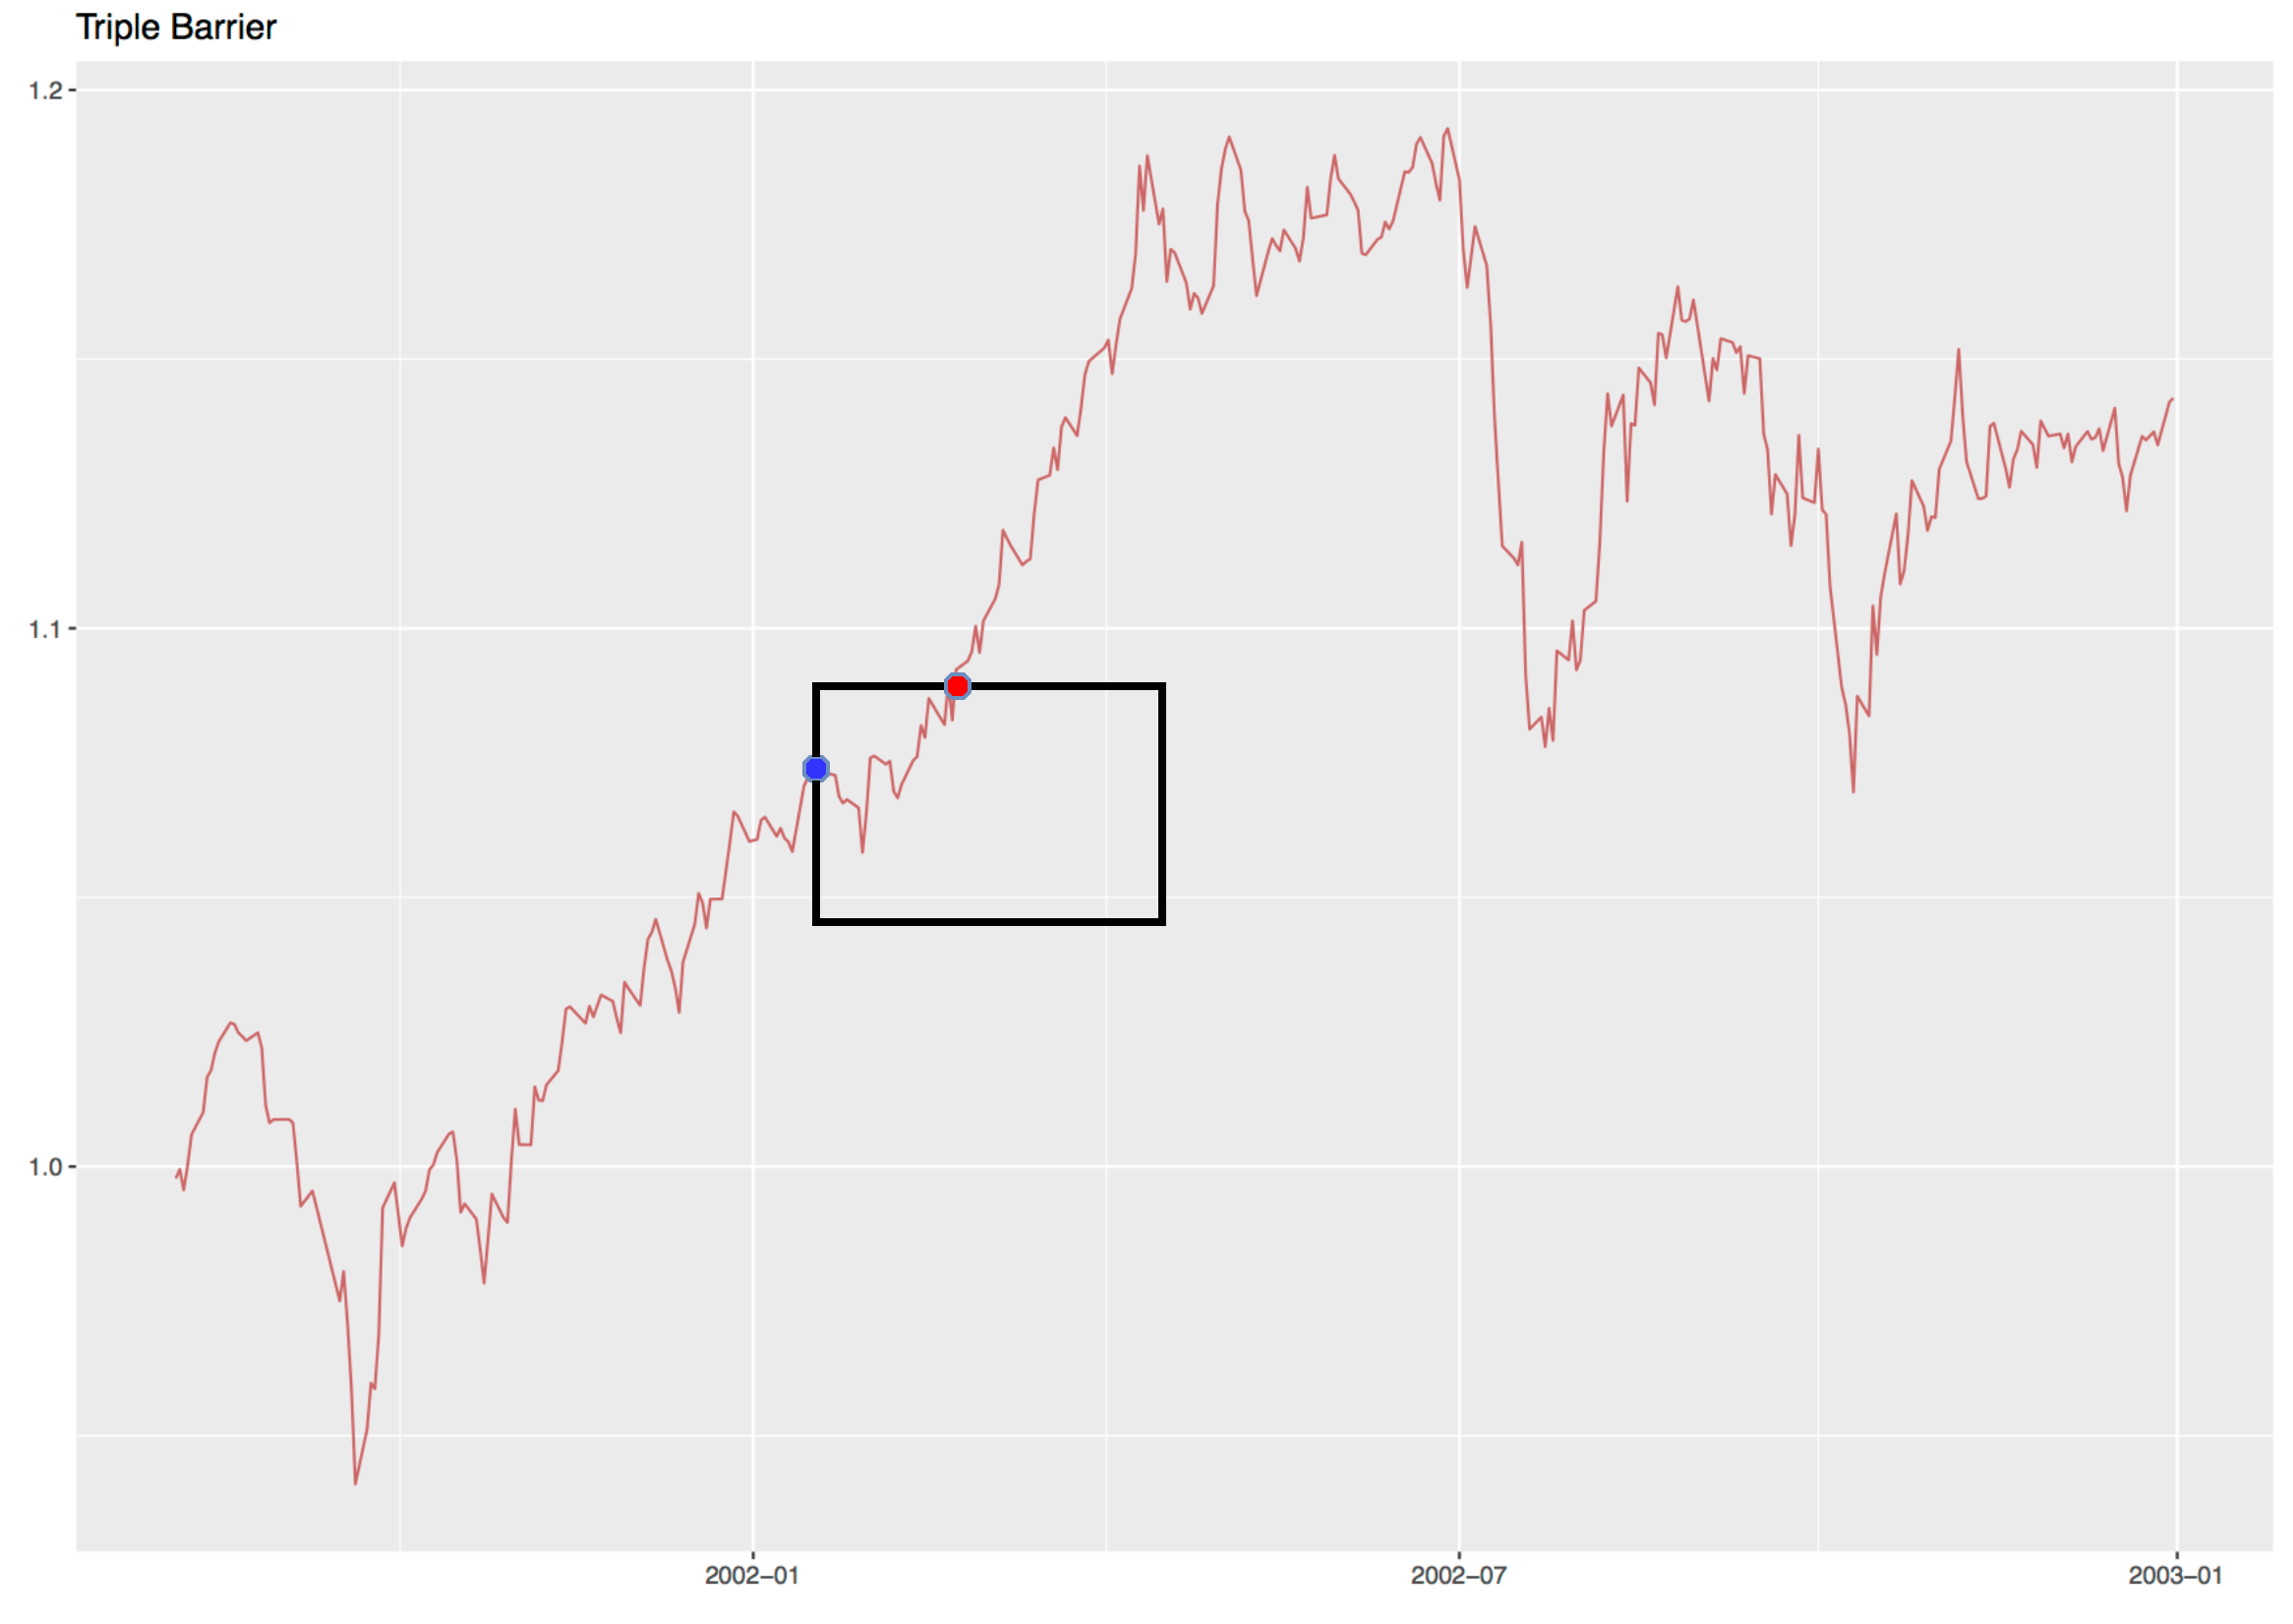
\includegraphics[width=.9\textwidth]
			{../img/tripleBarrierSide.png}
			\caption{Non-symmetrical horizontal barriers (Side $= 
			-1$)}
			\label{fig:tripleBarrierSide}
		\end{figure}

	\end{column}
	
	\end{columns}

\end{frame}	

\begin{frame}{Triple Barrier Method}

Noting $t_{\text{hit}},\ t_{\text{start}}$ as the time the barriers 
start and get hit, respectively, the realized return can be computed 
as:
	\begin{equation*}
		r_k = \left( \frac{p_{t_{\text{hit}}}}{p_{t_{\text{start}}}} 
		- 1 \right) \cdot \textbf{signal}_{t_{\text{start}}}
	\end{equation*}
	
	Combining everything, the observations are labeled as:
	\begin{equation*}
		y_k =
	    \begin{cases}
	      1 & \text{if}\ r_k > 0 \\
	      0 & \text{otherwise}
	    \end{cases}
	\end{equation*}

\end{frame}

\begin{frame}{Results}
\framesubtitle{Moving Average (MA) \& ML Models}

	\begin{columns}
		
		\begin{column}{.45\textwidth}
			\begin{figure}
			\centering
				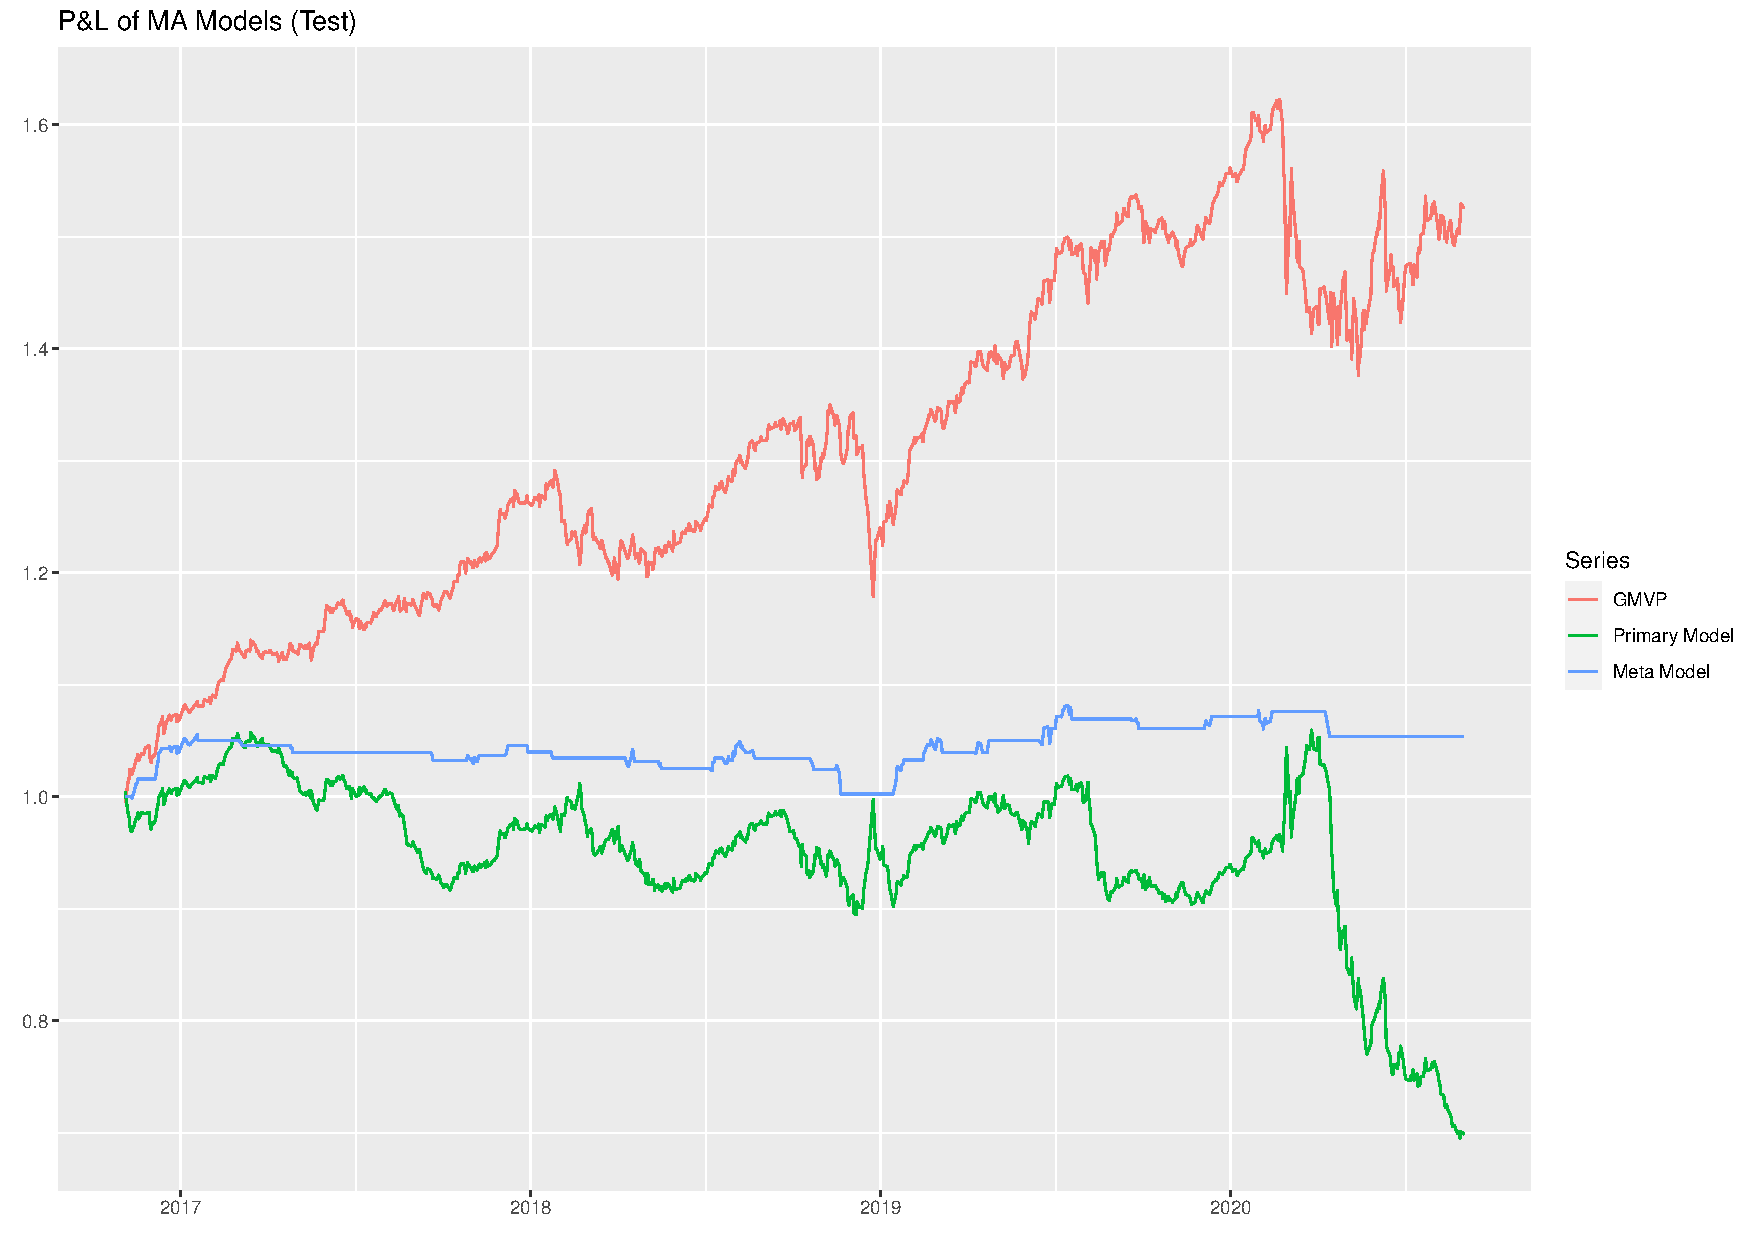
\includegraphics[scale=.2]{../img/Plots_MA_Test}
			\end{figure}
		
		
		\begin{table}[htbp]
			\tiny
			\centering
			\begin{tabular}{ |C{1cm}|C{2cm}|C{1.5cm}| }
				\hline
				Model & Max. Drawdown (Test) & SR (Test)\\
				\hline
				B\&H & 15.20\% & 0.9682\\ 
				M1 & 34.41\% & -0.7467\\ 
				MM & 5.02\% 	& 0.4887\\ 
				\hline
			\end{tabular}
		\end{table}

		\end{column}		
		
		\begin{column}{.45\textwidth}
			\begin{figure}
			\centering
				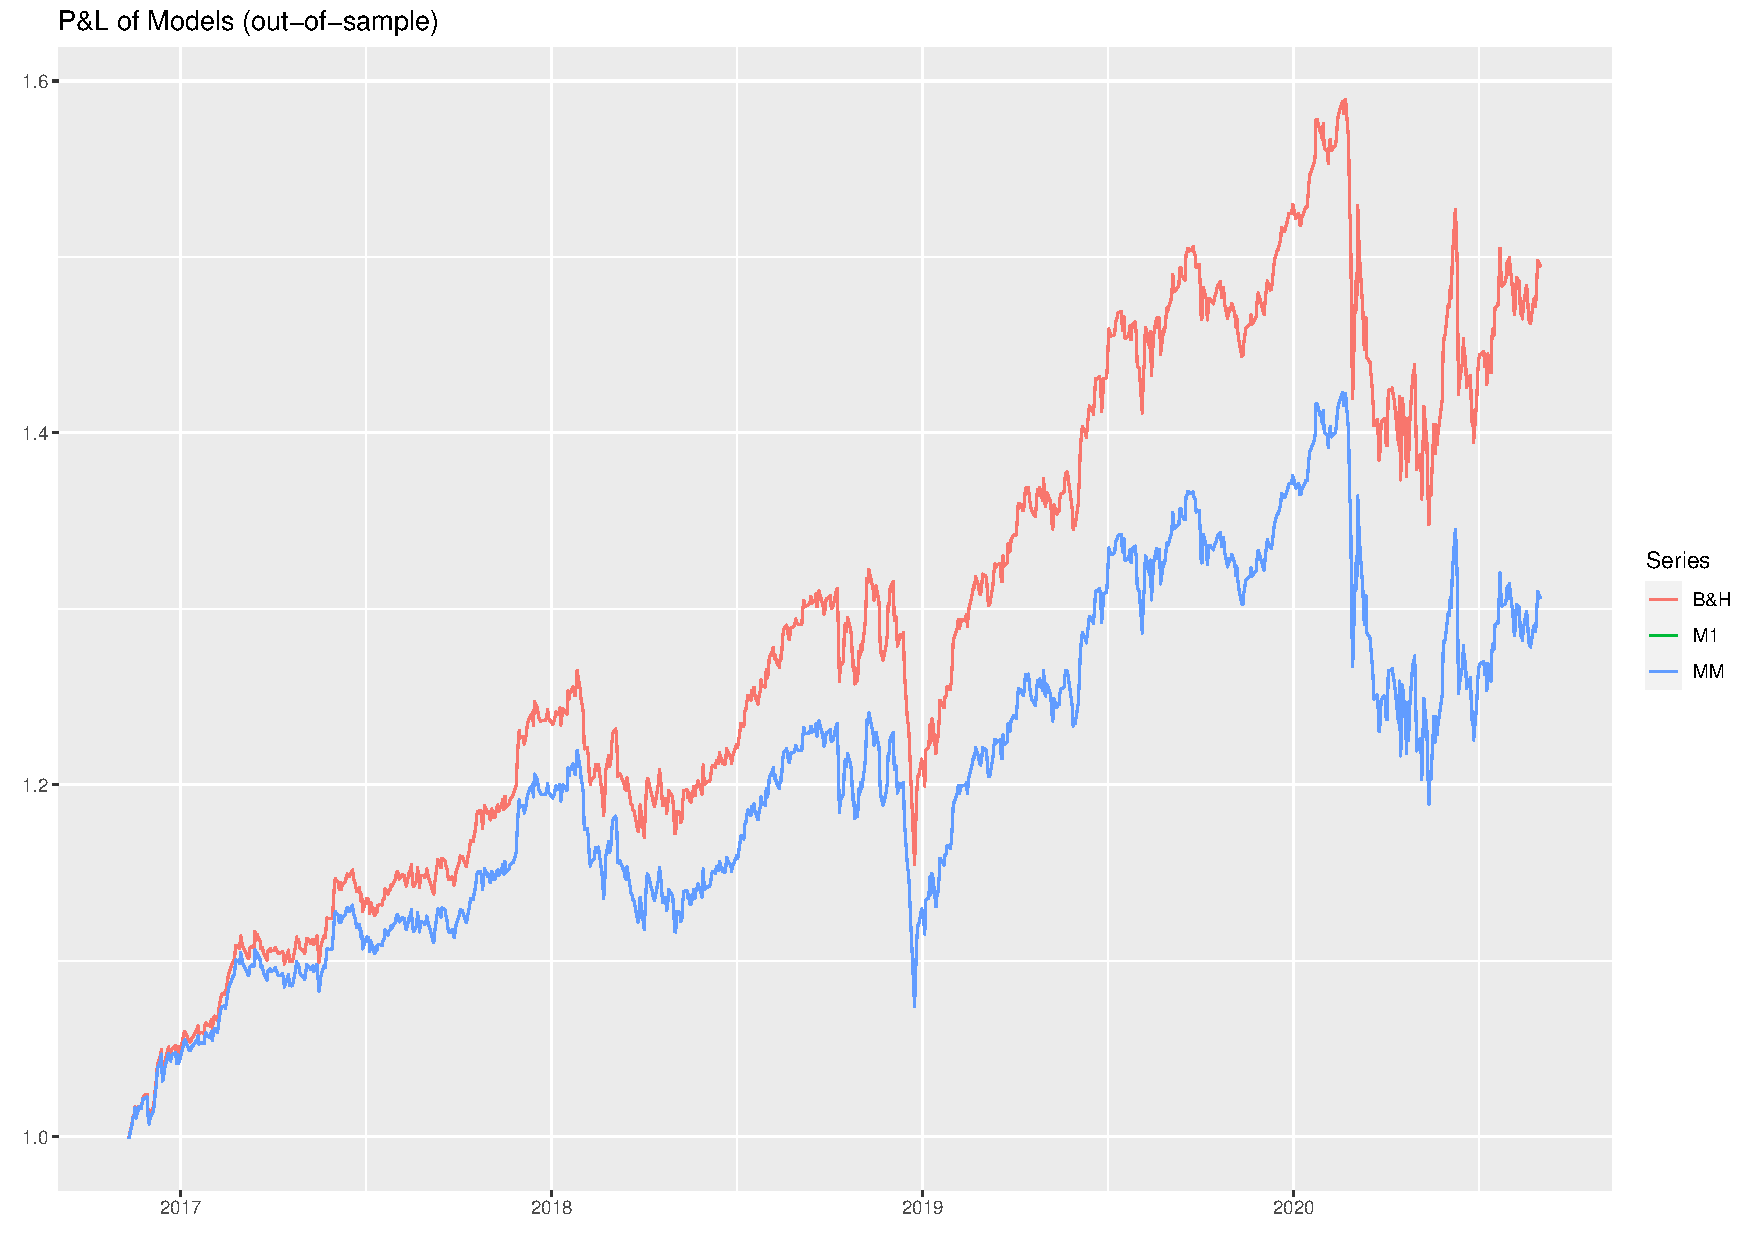
\includegraphics[scale=.2]{../img/Plots_ML_Test}
			\end{figure}
			
			\begin{table}[htbp]
			\tiny
			\centering
			\begin{tabular}{ |C{1cm}|C{2cm}|C{1.5cm}| }
				\hline
				Model & Max. Drawdown (Test) & SR (Test)\\
				\hline
				B\&H & 15.20\% & 0.9682\\ 
				M1 & 16.66\% & 0.7069\\ 
				MM & 14.57\% & 0.7302\\ 
				\hline
			\end{tabular}
			\end{table}			
			
		\end{column}		

	\end{columns}

	\vspace{.2cm}
	

\end{frame}

% \bibliography{references}

\end{document}
